% !TEX program = pdflatex
% Nonlinear Optics Assignment 7
\documentclass[UTF8,10pt,a4paper]{article}
\usepackage[scheme=plain]{ctex}
\newcommand{\CourseName}{Nonlinear Optics}
\newcommand{\CourseCode}{PHYS2202}
\newcommand{\Semester}{Spring, 2020}
\newcommand{\ProjectName}{Assignment 7}
\newcommand{\DueTimeType}{Due Time}
\newcommand{\DueTime}{17:00, May 27, 2020 (Tuesday)}
\newcommand{\StudentName}{陈稼霖}
\newcommand{\StudentID}{45875852}
\usepackage[vmargin=1in,hmargin=.5in]{geometry}
\usepackage{fancyhdr}
\usepackage{lastpage}
\usepackage{calc}
\pagestyle{fancy}
\fancyhf{}
\fancyhead[L]{\CourseName}
\fancyhead[C]{\ProjectName}
\fancyhead[R]{\StudentName}
\fancyfoot[R]{\thepage\ / \pageref{LastPage}}
\setlength\headheight{12pt}
\fancypagestyle{FirstPageStyle}{
    \fancyhf{}
    \fancyhead[L]{\CourseName\\
        \CourseCode\\
        \Semester}
    \fancyhead[C]{{\Huge\bfseries\ProjectName}\\
        \DueTimeType\ : \DueTime}
    \fancyhead[R]{Name : \makebox[\widthof{\StudentID}][s]{\StudentName}\\
        Student ID\@ : \StudentID\\
        Score : \underline{\makebox[\widthof{\StudentID}]{}}}
    \fancyfoot[R]{\thepage\ / \pageref{LastPage}}
    \setlength\headheight{36pt}
}
\usepackage{amsmath,amssymb,amsthm,bm}
\allowdisplaybreaks[4]
\newtheoremstyle{Problem}
{}
{}
{}
{}
{\bfseries}
{.}
{ }
{\thmname{#1}\thmnumber{ #2}\thmnote{ (#3)} Score: \underline{\qquad\qquad}}
\theoremstyle{Problem}
\newtheorem{prob}{Problem}
\newtheoremstyle{Solution}
{}
{}
{}
{}
{\bfseries}
{:}
{ }
{\thmname{#1}}
\makeatletter
\def\@endtheorem{\qed\endtrivlist\@endpefalse}
\makeatother
\theoremstyle{Solution}
\newtheorem*{sol}{Solution}
\providecommand{\abs}[1]{\left\lvert#1\right\rvert}
\usepackage{mathrsfs}
\usepackage{graphicx}
\usepackage{multirow}
\usepackage{listings}
\usepackage{listings}
\lstset{language=MATLAB,
numbers=left,
frame=single,
breaklines=true}
\begin{document}
\thispagestyle{FirstPageStyle}
\begin{prob}[(20 points) Nonlinear crystal orientation and length]
    Suppose that you have a pulsed Ti:sapphire laser system producing $100$ fs pulses at $800$ nm wavelength and you would like to generate terahertz pulses at $\sim 20$ THz ($15\,\mu$m wavelength). As a first step, you will convert the Ti:sapphire output to signal and idler beams in the infrared (frequencies $\omega_s$ and $\omega_i$), which you will then mix in an appropriate nonlinear crystal (e.g., GaSe) to generate the terahertz radiation by difference frequency mixing $\omega_s-\omega_i=\omega_{\text{THz}}$.

    You need to purchase a $\beta$-BBO (BBO=Ba$_2$B$_2$O$_4$, barium borate, symmetry group: $3m$) crystal to convert the $800$ nm light to the infrared. Suppose that your laser source produces pulses of the $800$ nm light in a TEM$_{00}$ spatial mode with an energy of $20\mu$J.

    Explain which type of phase matching (Type I or Type II) you should use to realize the most efficient conversion of the $800$ nm light, and then explain the orientation, length, and cross section of the BBO crystal.

    The following are some relevant parameters for BBO:
    \begin{enumerate}
        \item[1.] wavelength dispersion of the refractive indices:
        \begin{align}
            \nonumber n_O^2=&2.7405+\frac{0.0184}{\lambda^2-0.0179}-0.0155\lambda^2,\\
            n_E^2=&2.3730+\frac{0.0128}{\lambda^2-0.0156}-0.0044\lambda^2,
        \end{align}
        where $\lambda$ is in $\mu$m.
        \item[2.] Effective nonlinearity$^1$:
        \begin{align}
            \nonumber d_{\text{ooe}}=&d_{31}\sin\theta-d_{22}\cos\theta\sin 3\phi,\\
            \nonumber d_{\text{eoe}}=&d_{\text{oee}}=d_{22}\cos^2\theta\cos 3\phi,\\
            \nonumber d_{22}=&\pm(2.22\pm 0.09)\text{pm}/\text{V},\\
            d_{31}=&\pm(0.16\pm 0.08)\text{pm}/\text{V}.
        \end{align}
        \item[3.] Angular acceptance at $800$ nm $\sim$ $0.8$ mrad cm.
        \item[4.] Damage threshold for $1$ ps pulses at $1064$ nm $\sim 50\text{GW}/\text{cm}$. Suppose that the damage threshold for $100$ fs, $800$ nm pulses is the same.
    \end{enumerate}
\end{prob}
\begin{sol}
%     We first consider \textbf{the magnitude of the effective nonlinear susceptibility}. Here, we use symmetry of BBO to find the zero elements of the $2$nd-order electric-dipolar susceptibility and the dependency relations of between the non-zero elements. The point group of BBO is $3m$, whose symmetry operations are only a three-fold rotation and a mirror plane perpendicular to the rotation axis. Without loss of generality, we choose the three-fold rotation axis as $z$ axis.
%     \begin{enumerate}
%         \item \textbf{Mirror plane $m_{100}$}: Suppose we reflect the system by the mirror plane perpendicular to $(1,0,0)$. This operation can be represented by the matrix:
%         \begin{align}
%             R(m_{100})=\left(\begin{matrix}
%                 -1&0&0\\
%                 0&1&0\\
%                 0&0&1
%             \end{matrix}\right).
%         \end{align}
%         After the reflection, the $2$nd order electric dipolar susceptibility must satisfy
%         \begin{align}
%             \nonumber\chi_{\text{ED},\mu\alpha\beta}^{(2)}=&R_{\mu u}(m_{100})R_{\alpha a}(m_{100})R_{\beta b}(m_{100})\chi_{EQ,uab}\\
%             =&[\delta_{\mu x}+\delta_{\mu y}+\delta_{\mu z}][-\delta_{\alpha x}+\delta_{\alpha y}+\delta_{\alpha z}][-\delta_{\beta x}+\delta_{\beta y}+\delta_{\beta z}]\chi_{\text{ED},\mu\alpha\beta}.
%         \end{align}
%         According to the above equation, there are two kinds of cases:
%         \begin{itemize}
%             \item In \textbf{cases that the number of $x$ in $\{\mu,\alpha,\beta\}$ is odd}, we have
%             \begin{align}
%                 \chi_{\text{ED},\mu\alpha\beta}^{(2)}=-\chi_{\text{ED},\mu\alpha\beta}^{(2)},
%             \end{align}
%             so
%             \begin{align}
%                 \chi_{\text{ED},\mu\alpha\beta}^{(2)}=0.
%             \end{align}
%             \item In \textbf{cases that the number of $x$ in $\{\mu,\alpha,\beta\}$ is even}, we have
%             \begin{align}
%                 \chi_{\text{ED},\mu\alpha\beta}^{(2)}=\chi_{\text{ED},\mu\alpha\beta}^{(2)}.
%             \end{align}
%             This trivial equation can not provide any useful information for us.
%         \end{itemize}
%         The susceptibility elements $\chi_{\text{ED},\mu\alpha\beta}^{(2)}$ required by the symmetry operation $m_{100}$ to be zero are
%         \begin{gather*}
%             \chi_{\text{ED},xyy}^{(2)},\quad\chi_{\text{ED},xyz}^{(2)},\quad\chi_{\text{ED},xzy}^{(2)},\quad\chi_{\text{ED},xzz}^{(2)},\\
%             \chi_{\text{ED},yxy}^{(2)},\quad\chi_{\text{ED},yxz}^{(2)},\quad\chi_{\text{ED},zxy}^{(2)},\quad\chi_{\text{ED},zxz}^{(2)},\\
%             \chi_{\text{ED},yyx}^{(2)},\quad\chi_{\text{ED},yzx}^{(2)},\quad\chi_{\text{ED},zyx}^{(2)},\quad\chi_{\text{ED},zzx}^{(2)},\\
%             \chi_{\text{ED},xxx}^{(2)}.
%         \end{gather*}
%         \item Suppose we rotate the system by $\frac{2\pi}{3}$ about the $z$ axis counterclockwisely. This rotation can represented by the matrix:
%     \begin{align}
%         R(3_z)=\left(\begin{matrix}
%             \cos\frac{2\pi}{3}&-\sin\frac{2\pi}{3}&0\\
%             \sin\frac{2\pi}{3}&\cos\frac{2\pi}{3}&0\\
%             0&0&1
%         \end{matrix}\right)=\left(\begin{matrix}
%             \frac{1}{2}&-\frac{\sqrt{3}}{2}&0\\
%             \frac{\sqrt{3}}{2}&\frac{1}{2}&0\\
%             0&0&1
%         \end{matrix}\right).
%     \end{align}
%     Under this rotation, the $2$nd order electric dipolar susceptibility must satisfy
%     \begin{align}
%         \chi_{\text{ED},\mu\alpha\beta}^{(2)}=R_{\mu u}(3_z)R_{\alpha a}(3_z)R_{\beta b}(3_z)\chi_{\text{ED},uab}^{(2)}.
%     \end{align}
%     Since $\chi_{\text{ED},\mu\alpha\beta}$ is non-zero only if there are zero or two $x$ in $\{\mu,\alpha,\beta\}$,
%     \footnotesize
%     \begin{align}
%         \nonumber&\chi_{\text{ED},\mu\alpha\beta}^{(2)}=\sum_{u\in\{y,z\}}\sum_{a\in\{y,z\}}\sum_{b\in\{y,z\}}R_{\mu u}(3_z)R_{\alpha a}(3_z)R_{\beta b}(3_z)\chi_{\text{ED},uab}^{(2)}\\
%         &+\sum_{b\in\{y,z\}}R_{\mu x}(3_z)R_{\alpha x}(3_z)R_{\beta b}(3_z)\chi_{\text{ED},xx\beta}^{(2)}+\sum_{u\in\{y,z\}}R_{\mu u}(3_z)R_{\alpha x}(3_z)R_{\beta x}(3_z)\chi_{\text{ED},uxx}^{(2)}+\sum_{a\in\{y,z\}}R_{\mu x}(3_z)R_{\alpha a}(3_z)R_{\beta x}(3_z)\chi_{\text{ED},xax}^{(2)}.
%     \end{align}
%     \normalsize

%     The above equation can give $27$ relations of the $2$nd order electric dipolar susceptibility:
% \begin{itemize}
% \item For $u=x,\alpha=x,\beta=x$, we have
% \small\begin{align}
% \nonumber\chi_{\text{ED},xxx}^{(2)}=&\left(-\frac{\sqrt{3}}{2}\right)\left(-\frac{\sqrt{3}}{2}\right)\left(-\frac{\sqrt{3}}{2}\right)\chi_{\text{ED},yyy}^{(2)}\\
% &+\left[\left(-\frac{1}{2}\right)\left(-\frac{1}{2}\right)\left(-\frac{\sqrt{3}}{2}\right)\chi_{\text{ED},xxy}^{(2)}\right]+\left[\left(-\frac{\sqrt{3}}{2}\right)\left(-\frac{1}{2}\right)\left(-\frac{1}{2}\right)\chi_{\text{ED},yxx}^{(2)}\right]+\left[\left(-\frac{1}{2}\right)\left(-\frac{\sqrt{3}}{2}\right)\left(-\frac{1}{2}\right)\chi_{\text{ED},xyx}^{(2)}\right]
% \end{align}\normalsize
% \item For $u=x,\alpha=x,\beta=y$, we have
% \small\begin{align}
% \nonumber\chi_{\text{ED},xxy}^{(2)}=&\left(-\frac{\sqrt{3}}{2}\right)\left(-\frac{\sqrt{3}}{2}\right)\left(-\frac{1}{2}\right)\chi_{\text{ED},yyy}^{(2)}\\
% &+\left[\left(-\frac{1}{2}\right)\left(-\frac{1}{2}\right)\left(-\frac{1}{2}\right)\chi_{\text{ED},xxy}^{(2)}\right]+\left[\left(-\frac{\sqrt{3}}{2}\right)\left(-\frac{1}{2}\right)\frac{\sqrt{3}}{2}\chi_{\text{ED},yxx}^{(2)}\right]+\left[\left(-\frac{1}{2}\right)\left(-\frac{\sqrt{3}}{2}\right)\frac{\sqrt{3}}{2}\chi_{\text{ED},xyx}^{(2)}\right]
% \end{align}\normalsize
% \item For $u=x,\alpha=x,\beta=z$, we have
% \small\begin{align}
% \nonumber\chi_{\text{ED},xxz}^{(2)}=&\left(-\frac{\sqrt{3}}{2}\right)\left(-\frac{\sqrt{3}}{2}\right)1\chi_{\text{ED},yyz}^{(2)}\\
% &+\left[\left(-\frac{1}{2}\right)\left(-\frac{1}{2}\right)1\chi_{\text{ED},xxz}^{(2)}\right]
% \end{align}\normalsize
% \item For $u=x,\alpha=y,\beta=x$, we have
% \small\begin{align}
% \nonumber\chi_{\text{ED},xyx}^{(2)}=&\left(-\frac{\sqrt{3}}{2}\right)\left(-\frac{1}{2}\right)\left(-\frac{\sqrt{3}}{2}\right)\chi_{\text{ED},yyy}^{(2)}\\
% &+\left[\left(-\frac{1}{2}\right)\frac{\sqrt{3}}{2}\left(-\frac{\sqrt{3}}{2}\right)\chi_{\text{ED},xxy}^{(2)}\right]+\left[\left(-\frac{\sqrt{3}}{2}\right)\frac{\sqrt{3}}{2}\left(-\frac{1}{2}\right)\chi_{\text{ED},yxx}^{(2)}\right]+\left[\left(-\frac{1}{2}\right)\left(-\frac{1}{2}\right)\left(-\frac{1}{2}\right)\chi_{\text{ED},xyx}^{(2)}\right]
% \end{align}\normalsize
% \item For $u=x,\alpha=y,\beta=y$, we have
% \small\begin{align}
% \nonumber\chi_{\text{ED},xyy}^{(2)}=&\left(-\frac{\sqrt{3}}{2}\right)\left(-\frac{1}{2}\right)\left(-\frac{1}{2}\right)\chi_{\text{ED},yyy}^{(2)}\\
% &+\left[\left(-\frac{1}{2}\right)\frac{\sqrt{3}}{2}\left(-\frac{1}{2}\right)\chi_{\text{ED},xxy}^{(2)}\right]+\left[\left(-\frac{\sqrt{3}}{2}\right)\frac{\sqrt{3}}{2}\frac{\sqrt{3}}{2}\chi_{\text{ED},yxx}^{(2)}\right]+\left[\left(-\frac{1}{2}\right)\left(-\frac{1}{2}\right)\frac{\sqrt{3}}{2}\chi_{\text{ED},xyx}^{(2)}\right]
% \end{align}\normalsize
% \item For $u=x,\alpha=y,\beta=z$, we have
% \small\begin{align}
% \nonumber\chi_{\text{ED},xyz}^{(2)}=&\left(-\frac{\sqrt{3}}{2}\right)\left(-\frac{1}{2}\right)1\chi_{\text{ED},yyz}^{(2)}\\
% &+\left[\left(-\frac{1}{2}\right)\frac{\sqrt{3}}{2}1\chi_{\text{ED},xxz}^{(2)}\right]
% \end{align}\normalsize
% \item For $u=x,\alpha=z,\beta=x$, we have
% \small\begin{align}
% \nonumber\chi_{\text{ED},xzx}^{(2)}=&\left(-\frac{\sqrt{3}}{2}\right)1\left(-\frac{\sqrt{3}}{2}\right)\chi_{\text{ED},yzy}^{(2)}\\
% &+\left[\left(-\frac{1}{2}\right)1\left(-\frac{1}{2}\right)\chi_{\text{ED},xzx}^{(2)}\right]
% \end{align}\normalsize
% \item For $u=x,\alpha=z,\beta=y$, we have
% \small\begin{align}
% \nonumber\chi_{\text{ED},xzy}^{(2)}=&\left(-\frac{\sqrt{3}}{2}\right)1\left(-\frac{1}{2}\right)\chi_{\text{ED},yzy}^{(2)}\\
% &+\left[\left(-\frac{1}{2}\right)1\frac{\sqrt{3}}{2}\chi_{\text{ED},xzx}^{(2)}\right]
% \end{align}\normalsize
% \item For $u=x,\alpha=z,\beta=z$, we have
% \small\begin{align}
% \nonumber\chi_{\text{ED},xzz}^{(2)}=&\left(-\frac{\sqrt{3}}{2}\right)11\chi_{\text{ED},yzz}^{(2)}\\
% &
% \end{align}\normalsize
% \item For $u=y,\alpha=x,\beta=x$, we have
% \small\begin{align}
% \nonumber\chi_{\text{ED},yxx}^{(2)}=&\left(-\frac{1}{2}\right)\left(-\frac{\sqrt{3}}{2}\right)\left(-\frac{\sqrt{3}}{2}\right)\chi_{\text{ED},yyy}^{(2)}\\
% &+\left[\frac{\sqrt{3}}{2}\left(-\frac{1}{2}\right)\left(-\frac{\sqrt{3}}{2}\right)\chi_{\text{ED},xxy}^{(2)}\right]+\left[\left(-\frac{1}{2}\right)\left(-\frac{1}{2}\right)\left(-\frac{1}{2}\right)\chi_{\text{ED},yxx}^{(2)}\right]+\left[\frac{\sqrt{3}}{2}\left(-\frac{\sqrt{3}}{2}\right)\left(-\frac{1}{2}\right)\chi_{\text{ED},xyx}^{(2)}\right]
% \end{align}\normalsize
% \item For $u=y,\alpha=x,\beta=y$, we have
% \small\begin{align}
% \nonumber\chi_{\text{ED},yxy}^{(2)}=&\left(-\frac{1}{2}\right)\left(-\frac{\sqrt{3}}{2}\right)\left(-\frac{1}{2}\right)\chi_{\text{ED},yyy}^{(2)}\\
% &+\left[\frac{\sqrt{3}}{2}\left(-\frac{1}{2}\right)\left(-\frac{1}{2}\right)\chi_{\text{ED},xxy}^{(2)}\right]+\left[\left(-\frac{1}{2}\right)\left(-\frac{1}{2}\right)\frac{\sqrt{3}}{2}\chi_{\text{ED},yxx}^{(2)}\right]+\left[\frac{\sqrt{3}}{2}\left(-\frac{\sqrt{3}}{2}\right)\frac{\sqrt{3}}{2}\chi_{\text{ED},xyx}^{(2)}\right]
% \end{align}\normalsize
% \item For $u=y,\alpha=x,\beta=z$, we have
% \small\begin{align}
% \nonumber\chi_{\text{ED},yxz}^{(2)}=&\left(-\frac{1}{2}\right)\left(-\frac{\sqrt{3}}{2}\right)1\chi_{\text{ED},yyz}^{(2)}\\
% &+\left[\frac{\sqrt{3}}{2}\left(-\frac{1}{2}\right)1\chi_{\text{ED},xxz}^{(2)}\right]
% \end{align}\normalsize
% \item For $u=y,\alpha=y,\beta=x$, we have
% \small\begin{align}
% \nonumber\chi_{\text{ED},yyx}^{(2)}=&\left(-\frac{1}{2}\right)\left(-\frac{1}{2}\right)\left(-\frac{\sqrt{3}}{2}\right)\chi_{\text{ED},yyy}^{(2)}\\
% &+\left[\frac{\sqrt{3}}{2}\frac{\sqrt{3}}{2}\left(-\frac{\sqrt{3}}{2}\right)\chi_{\text{ED},xxy}^{(2)}\right]+\left[\left(-\frac{1}{2}\right)\frac{\sqrt{3}}{2}\left(-\frac{1}{2}\right)\chi_{\text{ED},yxx}^{(2)}\right]+\left[\frac{\sqrt{3}}{2}\left(-\frac{1}{2}\right)\left(-\frac{1}{2}\right)\chi_{\text{ED},xyx}^{(2)}\right]
% \end{align}\normalsize
% \item For $u=y,\alpha=y,\beta=y$, we have
% \small\begin{align}
% \nonumber\chi_{\text{ED},yyy}^{(2)}=&\left(-\frac{1}{2}\right)\left(-\frac{1}{2}\right)\left(-\frac{1}{2}\right)\chi_{\text{ED},yyy}^{(2)}\\
% &+\left[\frac{\sqrt{3}}{2}\frac{\sqrt{3}}{2}\left(-\frac{1}{2}\right)\chi_{\text{ED},xxy}^{(2)}\right]+\left[\left(-\frac{1}{2}\right)\frac{\sqrt{3}}{2}\frac{\sqrt{3}}{2}\chi_{\text{ED},yxx}^{(2)}\right]+\left[\frac{\sqrt{3}}{2}\left(-\frac{1}{2}\right)\frac{\sqrt{3}}{2}\chi_{\text{ED},xyx}^{(2)}\right]
% \end{align}\normalsize
% \item For $u=y,\alpha=y,\beta=z$, we have
% \small\begin{align}
% \nonumber\chi_{\text{ED},yyz}^{(2)}=&\left(-\frac{1}{2}\right)\left(-\frac{1}{2}\right)1\chi_{\text{ED},yyz}^{(2)}\\
% &+\left[\frac{\sqrt{3}}{2}\frac{\sqrt{3}}{2}1\chi_{\text{ED},xxz}^{(2)}\right]
% \end{align}\normalsize
% \item For $u=y,\alpha=z,\beta=x$, we have
% \small\begin{align}
% \nonumber\chi_{\text{ED},yzx}^{(2)}=&\left(-\frac{1}{2}\right)1\left(-\frac{\sqrt{3}}{2}\right)\chi_{\text{ED},yzy}^{(2)}\\
% &+\left[\frac{\sqrt{3}}{2}1\left(-\frac{1}{2}\right)\chi_{\text{ED},xzx}^{(2)}\right]
% \end{align}\normalsize
% \item For $u=y,\alpha=z,\beta=y$, we have
% \small\begin{align}
% \nonumber\chi_{\text{ED},yzy}^{(2)}=&\left(-\frac{1}{2}\right)1\left(-\frac{1}{2}\right)\chi_{\text{ED},yzy}^{(2)}\\
% &+\left[\frac{\sqrt{3}}{2}1\frac{\sqrt{3}}{2}\chi_{\text{ED},xzx}^{(2)}\right]
% \end{align}\normalsize
% \item For $u=y,\alpha=z,\beta=z$, we have
% \small\begin{align}
% \nonumber\chi_{\text{ED},yzz}^{(2)}=&\left(-\frac{1}{2}\right)11\chi_{\text{ED},yzz}^{(2)}\\
% &
% \end{align}\normalsize
% which means that
% \begin{align}
%     \chi_{\text{ED},yzz}^{(2)}=0,
% \end{align}
% and thus
% \begin{align}
%     \chi_{\text{ED},xzz}^{(2)}=0.
% \end{align}
% \item For $u=z,\alpha=x,\beta=x$, we have
% \small\begin{align}
% \nonumber\chi_{\text{ED},zxx}^{(2)}=&1\left(-\frac{\sqrt{3}}{2}\right)\left(-\frac{\sqrt{3}}{2}\right)\chi_{\text{ED},zyy}^{(2)}\\
% &+\left[1\left(-\frac{1}{2}\right)\left(-\frac{1}{2}\right)\chi_{\text{ED},zxx}^{(2)}\right]
% \end{align}\normalsize
% \item For $u=z,\alpha=x,\beta=y$, we have
% \small\begin{align}
% \nonumber\chi_{\text{ED},zxy}^{(2)}=&1\left(-\frac{\sqrt{3}}{2}\right)\left(-\frac{1}{2}\right)\chi_{\text{ED},zyy}^{(2)}\\
% &+\left[1\left(-\frac{1}{2}\right)\frac{\sqrt{3}}{2}\chi_{\text{ED},zxx}^{(2)}\right]
% \end{align}\normalsize
% \item For $u=z,\alpha=x,\beta=z$, we have
% \small\begin{align}
% \nonumber\chi_{\text{ED},zxz}^{(2)}=&1\left(-\frac{\sqrt{3}}{2}\right)1\chi_{\text{ED},zyz}^{(2)}\\
% &
% \end{align}\normalsize
% \item For $u=z,\alpha=y,\beta=x$, we have
% \small\begin{align}
% \nonumber\chi_{\text{ED},zyx}^{(2)}=&1\left(-\frac{1}{2}\right)\left(-\frac{\sqrt{3}}{2}\right)\chi_{\text{ED},zyy}^{(2)}\\
% &+\left[1\frac{\sqrt{3}}{2}\left(-\frac{1}{2}\right)\chi_{\text{ED},zxx}^{(2)}\right]
% \end{align}\normalsize
% \item For $u=z,\alpha=y,\beta=y$, we have
% \small\begin{align}
% \nonumber\chi_{\text{ED},zyy}^{(2)}=&1\left(-\frac{1}{2}\right)\left(-\frac{1}{2}\right)\chi_{\text{ED},zyy}^{(2)}\\
% &+\left[1\frac{\sqrt{3}}{2}\frac{\sqrt{3}}{2}\chi_{\text{ED},zxx}^{(2)}\right]
% \end{align}\normalsize
% \item For $u=z,\alpha=y,\beta=z$, we have
% \small\begin{align}
% \nonumber\chi_{\text{ED},zyz}^{(2)}=&1\left(-\frac{1}{2}\right)1\chi_{\text{ED},zyz}^{(2)}\\
% &
% \end{align}\normalsize
% which means that
% \begin{align}
%     \chi_{\text{ED},zyz}^{(2)}=0,
% \end{align}
% and thus
% \begin{align}
%     \chi_{\text{ED},zxz}^{(2)}=0.
% \end{align}
% \item For $u=z,\alpha=z,\beta=x$, we have
% \small\begin{align}
% \nonumber\chi_{\text{ED},zzx}^{(2)}=&11\left(-\frac{\sqrt{3}}{2}\right)\chi_{\text{ED},zzy}^{(2)}\\
% &
% \end{align}\normalsize
% \item For $u=z,\alpha=z,\beta=y$, we have
% \small\begin{align}
% \nonumber\chi_{\text{ED},zzy}^{(2)}=&11\left(-\frac{1}{2}\right)\chi_{\text{ED},zzy}^{(2)}\\
% &
% \end{align}\normalsize
% which means that
% \begin{align}
%     \chi_{\text{ED},zzy}^{(2)}=0,
% \end{align}
% and thus
% \begin{align}
%     \chi_{\text{ED},zzx}^{(2)}=0.
% \end{align}
% \item For $u=z,\alpha=z,\beta=z$, we have
% \small\begin{align}
% \nonumber\chi_{\text{ED},zzz}^{(2)}=&111\chi_{\text{ED},zzz}^{(2)}\\
% &
% \end{align}\normalsize
% \end{itemize}
%     \end{enumerate}
%     As a result of symmetry, there are $16$ susceptibility elements required to be zero, and only $2$ elements are truly independent. Using the dependency relations derived above and the given effective nonlinearity, the nonlinear polarization can be expressed as
%     \begin{align}
%         \left(\begin{matrix}
%             P_x\\
%             P_y\\
%             P_z
%         \end{matrix}\right)=\left(\begin{matrix}
%             0&0&0&0&d_{31}&-d_{22}\\
%             -d_{22}&d_{22}&0&d_{31}&0&0\\
%             d_{31}&d_{31}&d_{33}&0&0&0
%         \end{matrix}\right)\left(\begin{matrix}
%             E_x^2\\
%             E_y^2\\
%             E_z^2\\
%             2E_yE_z\\
%             2E_zE_x\\
%             2E_xE_y
%         \end{matrix}\right).
%     \end{align}

    We first consider the \textbf{the phase matching condition}. The conservation of energy requires that the sum of the frequencies of the signal and the idler beams should be equal to the frequencies of the input laser pump:
    \begin{align}
        \omega_s+\omega_i=\omega_p\equiv\frac{2\pi c}{800\text{nm}}=2.356\times 10^{15}\text{rad}/\text{s}.
    \end{align}
    To generate terahertz radiation by difference frequency mixing, the difference of the signal and idler beams should be equal to the frequency of the terahertz radiation:
    \begin{align}
        \omega_s-\omega_i=\omega_{\text{THz}}=2\pi\times 20\times 10^{12}\text{rad}/\text{s}=1.257\times 10^{14}\text{rad}/\text{s}.
    \end{align}
    Using the above two equations, we get the frequencies of the signal and the idler beams:
    \begin{align}
        \omega_s=&1.241\times 10^{15}\text{rad}/\text{s},\\
        \omega_i=&1.115\times 10^{15}\text{rad}/\text{s}.
    \end{align}

    Since the symmetry group of BBO is $3m$, it belongs to trigonal crystal system and thus is a uniaxial crystal. Since we set the three-fold axis as $z$ axis, the $z$ axis is the optic axis. The dispersion relations in terms of frequency are:
    \begin{align}
        n_O=&\left[2.7405+\frac{0.0184}{\left(\frac{2\pi c}{\omega}\times 10^6\right)^2-0.0179}-0.0155\left(\frac{2\pi c}{\omega}\times 10^6\right)^2\right]^{1/2},\\
        n_E=&\left[2.3730+\frac{0.0128}{\left(\frac{2\pi c}{\omega}\times 10^6\right)^2-0.0156}-0.0044\left(\frac{2\pi c}{\omega}\times 10^6\right)^2\right]^{1/2},
    \end{align}
    where $\omega$ is in rad/s.\\
    Using the two formulas above, we can calculate some refractive indices for later reference:
    \begin{align}
        n_O(\omega_p)=&1.661,\\
        n_O(\omega_s)=&1.647,\\
        n_O(\omega_i)=&1.644,\\
        n_E(\omega_p)=&1.546,\\
        n_E(\omega_s)=&1.539,\\
        n_E(\omega_i)=&1.538.
    \end{align}

    The phase matching condition of the process converting the input laser pump to the signal and the idler beams is
    \begin{gather}
        k(\omega_p)=k(\omega_1)+k(\omega_2),\\
        \Longrightarrow n(\omega_p)\omega_p=n(\omega_s)\omega_s+n(\omega_i)\omega_i.
    \end{gather}

    To see which type(s) of phase matching works, we examine all the combinations of polarization directions of the input and the output fields:
    \begin{enumerate}
        \item \textbf{Type I phase matching} (i.e., the polarization directions of the signal and the idler beams are the same, while the polarization direction of the input laser pump is orthogonal to them):
        \begin{enumerate}
            \item \textbf{Signal \& idler: ordinary; pump: ordinary}:
            \begin{gather}
                n(\omega_s)=n_O(\omega_s)=1.647,\\
                n(\omega_i)=n_O(\omega_i)=1.644,\\
                \Longrightarrow n(\omega_s)\omega_s+n(\omega_i)\omega_i=3.877\times 10^{15}\text{rad}/\text{s}.
            \end{gather}
            \begin{gather}
                n(\omega_p)=n_O(\omega_p)=1.661,\\
                \Longrightarrow n(\omega_p)\omega_p=3.915\times 10^{15}\text{rad}/\text{s}.
            \end{gather}
            Since $3.915\times 10^{15}\text{rad}/\text{s}\neq 3.877\times 10^{15}\text{rad}/\text{s}$, the phase matching condition does not hold under this combination of the input and the output polarization directions.
            \item \textbf{Signal \& idler: ordinary; pump: extraordinary}:
            \begin{gather}
                n(\omega_s)=n_O(\omega_s)=1.647,\\
                n(\omega_i)=n_O(\omega_i)=1.644,\\
                \Longrightarrow n(\omega_s)\omega_s+n(\omega_i)\omega_i=3.877\times 10^{15}\text{rad}/\text{s}.
            \end{gather}
            \begin{gather}
                1.546=n_E(\omega_p)\leq n(\omega_p)\leq n_O(\omega_p)=1.661,\\
                \Longrightarrow 3.643\times 10^{15}\text{rad}/\text{s}\leq n(\omega_p)\omega_p\leq 3.915\times 10^{15}\text{rad}/\text{s}.
            \end{gather}
            Since $3.643\times 10^{15}\text{rad}/\text{s}\leq 3.877\times 10^{15}\text{rad}/\text{s}\leq 3.915\times 10^{15}\text{rad}/\text{s}$, we can tune the angle $\theta$ between the beams and the optic axis of the crystal to achieve the phase matching condition.\\
            We are now to look for the angle $\theta$ that enables the phase matching condition. The refractive indices of the three beams in terms of $\theta$ are
            \begin{align}
                n(\omega_s,\theta)=&\left[\left(\frac{\cos\theta}{n_O(\omega_s)}\right)^2+\left(\frac{\sin\theta}{n_E(\omega_s)}\right)^2\right]^{-1/2},\\
                n(\omega_i,\theta)=&\left[\left(\frac{\cos\theta}{n_O(\omega_i)}\right)^2+\left(\frac{\sin\theta}{n_E(\omega_i)}\right)^2\right]^{-1/2},\\
                n(\omega_p,\theta)=&\left[\left(\frac{\cos\theta}{n_O(\omega_p)}\right)^2+\left(\frac{\sin\theta}{n_E(\omega_p)}\right)^2\right]^{-1/2}.
            \end{align}
            The phase matching condition can be rewritten as
            \begin{align}
                n(\omega_p,\theta)\omega_p-n(\omega_s,\theta)\omega_s-n(\omega_i,\theta)\omega_i=0.
            \end{align}
            Solving the above equation, or plotting the curve of function $f(\theta)=n(\omega_p,\theta)\omega_p-n(\omega_s,\theta)\omega_s-n(\omega_i,\theta)\omega_i$ and finding its intersection with the horizontal axis as shown in figure \ref{phase-matching-I-eoo}, we get the angle that enables the phase matching condition, $\theta=0.3608$ rad.
            \begin{figure}[h]
                \centering
                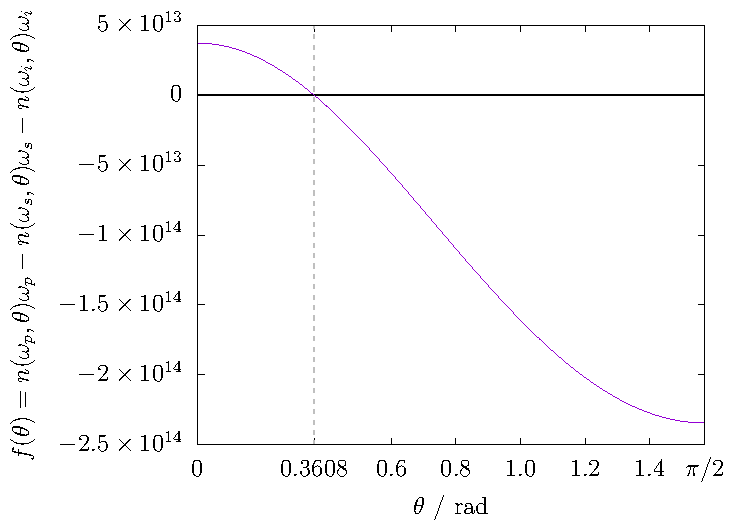
\includegraphics[width=.5\textwidth]{phase-matching-I-eoo.pdf}
                \caption{Curve of function $f(\theta)=n(\omega_p,\theta)\omega_p-n(\omega_s,\theta)\omega_s-n(\omega_i,\theta)\omega_i$ under the combination of: signal \& idler: ordinary; pump: extraordinary}
                \label{phase-matching-I-eoo}
            \end{figure}

            Under this combination of the input and the output polarization direction, the effective nonlinearity is
            \begin{align}
                d_{eoo}=d_{31}\sin\theta-d_{22}\cos\theta\sin 3\phi,
            \end{align}
            and its maximum is
            \begin{align}
                (d_{eoo})_{\max}=d_{ooe}(\theta=0.3608,\phi=\frac{(2m+1)\pi}{3},m\in\mathbb{Z})=2.135\text{pm}/\text{V}.
            \end{align}
            \item \textbf{Signal \& idler: extraordinary; pump: ordinary}:
            \begin{gather}
                1.539=n_E(\omega_s)\leq n(\omega_s)\leq n_O(\omega_s)=1.661,\\
                1.538=n_E(\omega_i)\leq n(\omega_i)\leq n_O(\omega_i)=1.644,\\
                \Longrightarrow 3.625\times 10^{15}\text{rad}/\text{s}\leq n(\omega_s)\omega_s+n(\omega_i)\omega_i\leq 3.877\times 10^{15}\text{rad}/\text{s}.
            \end{gather}
            \begin{gather}
                n(\omega_p)=n_O(\omega)=1.661,\\
                \Longrightarrow n(\omega_p)\omega_p=3.915\times 10^{15}\text{rad}/\text{s}.
            \end{gather}
            Since $3.915\times 10^{15}\text{rad}/\text{s}\notin[3.625\times 10^{15}\text{rad}/\text{s},3.877\times 10^{15}\text{rad}/\text{s}]$, we can not tune angle $\theta$ to achieve the phase matching condition.\\
        \item \textbf{Signal \& idler: extraordinary; pump: extraordinary}:
            \begin{gather}
                1.539=n_E(\omega_s)\leq n(\omega_s)\leq n_O(\omega_s)=1.661,\\
                1.538=n_E(\omega_i)\leq n(\omega_i)\leq n_O(\omega_i)=1.644,\\
                \Longrightarrow 3.625\times 10^{15}\text{rad}/\text{s}\leq n(\omega_s)\omega_s+n(\omega_i)\omega_i\leq 3.877\times 10^{15}\text{rad}/\text{s}.
            \end{gather}
            \begin{gather}
                1.546=n_E(\omega_p)\leq n(\omega_p)\leq n_O(\omega_p)=1.661,\\
                \Longrightarrow 3.643\times 10^{15}\text{rad}/\text{s}\leq n(\omega_p)\omega_p\leq 3.915\times 10^{15}\text{rad}/\text{s}.
            \end{gather}
            $[3.625\times 10^{15}\text{rad}/\text{s},3.877\times 10^{15}\text{rad}/\text{s}]\cap[3.643\times 10^{15}\text{rad}/\text{s},3.915\times 10^{15}\text{rad}/\text{s}]\neq\emptyset$, but the curve of function $f(\theta)=n(\omega_p,\theta)\omega_p-n(\omega_s,\theta)\omega_s-n(\omega_i,\theta)\omega_i$ has no intersection with the horizontal axis as shown in figure \ref{phase-matching-I-eee}, so under this combination of the input and the output polarization directions, there is no such an angle satisfying the phase matching condition.
            \begin{figure}[h]
                \centering
                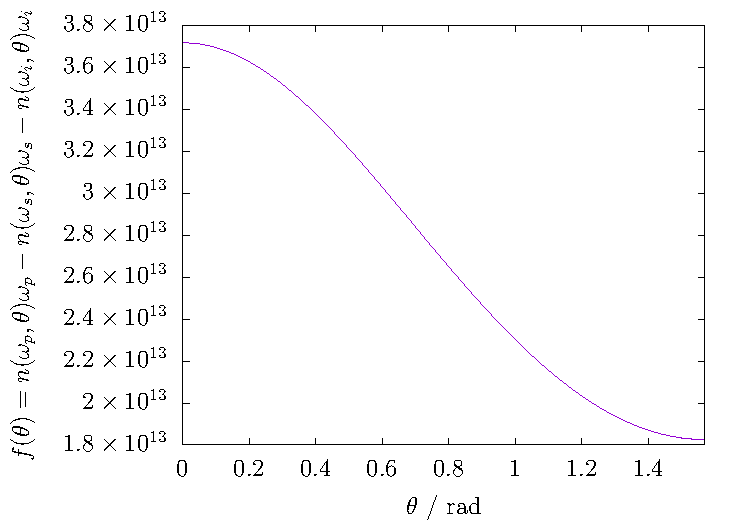
\includegraphics[width=.5\textwidth]{phase-matching-I-eee.pdf}
                \caption{Curve of function $f(\theta)=n(\omega_p,\theta)\omega_p-n(\omega_s,\theta)\omega_s-n(\omega_i,\theta)\omega_i$ given the combination: Signal \& idler: extraordinary; pump: extraordinary.}
                \label{phase-matching-I-eee}
            \end{figure}
        \end{enumerate}
        \item \textbf{Type II phase matching} (i.e., the polarization direction of the signal and the idler beams are orthogonal to each other):
        \begin{enumerate}
            \item \textbf{Signal: ordinary; idler: extraordinary; pump: ordinary}:
            \begin{gather}
                n(\omega_s)=n_O(\omega)=1.647,\\
                1.538=n_E(\omega_i)\leq n(\omega_i)\leq n_O(\omega_i)=1.644,\\
                \Longrightarrow 3.759\times 10^{15}\text{rad}/\text{s}\leq n(\omega_s)\omega_s+n(\omega_i)\omega_i\leq 3.877\times 10^{15}\text{rad}/\text{s}.
            \end{gather}
            \begin{gather}
                n(\omega_p)=n_O(\omega)=1.661,\\
                \Longrightarrow n(\omega_p)\omega_p=3.915\times 10^{15}\text{rad}/\text{s}.
            \end{gather}
            Since $3.915\times 10^{15}\text{rad}/\text{s}\notin[3.759\times 10^{15}\text{rad}/\text{s},3.877\times 10^{15}\text{rad}/\text{s}]$, we can not tune angle $\theta$ to achieve the phase matching condition.
            \item \textbf{Signal: ordinary; idler: extraordinary; pump: extraordinary}:
            \begin{gather}
                n(\omega_s)=n_O(\omega)=1.647,\\
                1.538=n_E(\omega_i)\leq n(\omega_i)\leq n_O(\omega_i)=1.644,\\
                \Longrightarrow 3.759\times 10^{15}\text{rad}/\text{s}\leq n(\omega_s)\omega_s+n(\omega_i)\omega_i\leq 3.877\times 10^{15}\text{rad}/\text{s}.
            \end{gather}
            \begin{gather}
                1.546=n_E(\omega_p)\leq n(\omega_p)\leq n_O(\omega_p)=1.661,\\
                \Longrightarrow 3.643\times 10^{15}\text{rad}/\text{s}\leq n(\omega_p)\omega_p\leq 3.915\times 10^{15}\text{rad}/\text{s}.
            \end{gather}
            Since $[3.759\times 10^{15}\text{rad}/\text{s},3.877\times 10^{15}\text{rad}/\text{s}]\cap[3.643\times 10^{15}\text{rad}/\text{s},3.915\times 10^{15}\text{rad}/\text{s}]\neq\emptyset$, we may find an angle $\theta$ satisfying the phase matching condition.\\
            To find the angle satisfying the phase matching condition, we plot he curve of the function $f(\theta)=n(\omega_p,\theta)\omega_p-n(\omega_s,\theta)\omega_s-n(\omega_i,\theta)\omega_i$ and find it has an intersection with the horizontal axis at $\theta=0.4912$ rad as shown in figure \ref{phase-matching-eoe}.
            \begin{figure}[h]
                \centering
                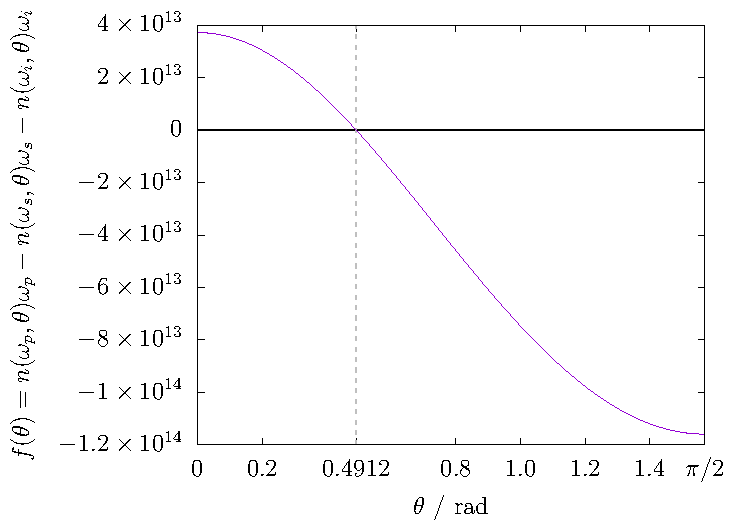
\includegraphics[width=.5\textwidth]{phase-matching-II-eoe.pdf}
                \caption{Curve of function $f(\theta)=n(\omega_p,\theta)\omega_p-n(\omega_s,\theta)\omega_s-n(\omega_i,\theta)\omega_i$ given the combination (Signal: ordinary; idler: extraordinary; pump: extraordinary)}
                \label{phase-matching-eoe}
            \end{figure}

            Under this combination of the input and the output polarization direction, the effective nonlinearity is
            \begin{align}
                d_{eoe}=d_{22}\cos^2\theta\cos 3\phi,
            \end{align}
            and its maximum is
            \begin{align}
                (d_{eoe})_{\max}=d_{oee}(\theta=0.4912,\phi=\frac{(2m+1)\pi}{6},m\in\mathbb{Z})=1.726\text{pm}/\text{V}.
            \end{align}
            \item \textbf{Signal: extraordinary; idler: ordinary; pump: ordinary}:
            \begin{gather}
                1.539=n_E(\omega_s)\leq n(\omega_s)\leq n_O(\omega_s)=1.647,\\
                n(\omega_i)=n_O(\omega_i)=1.644,\\
                \Longrightarrow 3.743\times 10^{15}\text{rad}/\text{s}\leq n(\omega_s)\omega_s+n(\omega_i)\omega_i\leq 3.877\times 10^{15}\text{rad}/\text{s}.
            \end{gather}
            \begin{gather}
                n(\omega_p)=\omega_O(\omega_p)=1.661,\\
                \Longrightarrow n(\omega_p)\omega_p=3.915\times 10^{15}\text{rad}/\text{s}.
            \end{gather}
            Since $3.915\times 10^{15}\text{rad}/\text{s}\notin[3.743\times 10^{15}\text{rad}/\text{s},3.877\times 10^{15}\text{rad}/\text{s}]$, we can not tune the angle $\theta$ to achieve the phase matching condition.
            \item \textbf{Signal: extraordinary; idler: ordinary; pump: extraordinary}:
            \begin{gather}
                1.539=n_E(\omega_s)\leq n(\omega_s)\leq n_O(\omega_s)=1.647,\\
                n(\omega_i)=n_O(\omega_i)=1.644,\\
                \Longrightarrow 3.743\times 10^{15}\text{rad}/\text{s}\leq n(\omega_s)\omega_s+n(\omega_i)\omega_i\leq 3.877\times 10^{15}\text{rad}/\text{s}.
            \end{gather}
            \begin{gather}
                1.546=n_E(\omega_p)\leq n(\omega_p)\leq n_O(\omega_p)=1.661,\\
                \Longrightarrow 3.643\times 10^{15}\text{rad}/\text{s}\leq n(\omega_p)\omega_p\leq 3.915\times 10^{15}\text{rad}/\text{s}.
            \end{gather}
            Since $[3.643\times 10^{15}\text{rad}/\text{s},3.915\times 10^{15}\text{rad}/\text{s}]\cap[3.743\times 10^{15}\text{rad}/\text{s},3.877\times 10^{15}\text{rad}/\text{s}]$, we may find an angle $\theta$ satisfying the phase matching condition.\\
            To find the angle satisfying the phase matching condition, we plot the curve of function $f(\theta)=n(\omega_p,\theta)\omega_p-n(\omega_s,\theta)\omega_s-n(\omega_i,\theta)\omega_i$ and find it has an intersection with the horizontal axis at $\theta=0.5222$ rad as shown in figure \ref{phase-matching-II-eeo}.
            \begin{figure}[h]
                \centering
                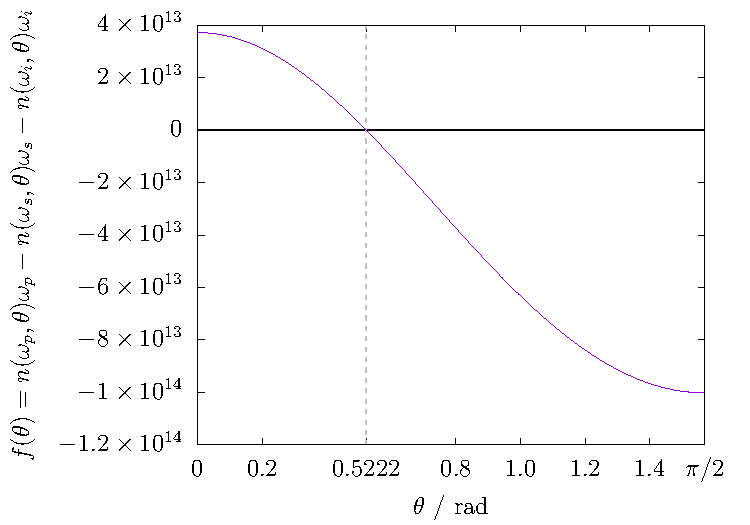
\includegraphics[width=.5\textwidth]{phase-matching-II-eeo.pdf}
                \caption{Curve of function $f(\theta)=n(\omega_p,\theta)\omega_p-n(\omega_s,\theta)\omega_s-n(\omega_i,\theta)\omega_i$ given the combination (Signal: extraordinary; idler: ordinary; pump: extraordinary)}
                \label{phase-matching-II-eeo}
            \end{figure}

            Under this combination of the input and the output polarization directions, the effective nonlinearity is
            \begin{align}
                d_{eeo}=d_{22}\cos^2\theta\cos 3\phi,
            \end{align}
            and its maximum is
            \begin{align}
                (d_{eeo})_{\max}=d_{eeo}(\theta=0.5222,\phi=\frac{(2m+1)\pi}{6},m\in\mathbb{Z})=1.668\text{pm}/\text{V}.
            \end{align}
        \end{enumerate}
    \end{enumerate}

    Among the combinations above, the type I phase matching (signal \& idler: ordinary; pump: extraordinary; $\theta=0.3608$ rad, $\phi=\frac{(2m+1)\pi}{3},m\in\mathbb{Z}$) has the maximum effective nonlinear coefficient and thus can realize the most efficient conversion of the $800$ nm light.

    We then consider the \textbf{damage} threshold of BBO. To avoid the input laser pulse's damage on the crystal, we can not focus the beam too tightly. The input laser pulse's instantaneous power is
    \begin{align}
        P=\frac{20\times 10^{-6}\text{J}}{100\times 10^{-15}s}=2\times 10^8\text{W}.
    \end{align}
    The power per unit area at the position of the waist (where the power density is the maximum) should not exceed the damage threshold:
    \begin{align}
        I=\frac{2P}{\pi w^2(0)}=\frac{2P}{\pi w_0^2}\leq 50\times 10^9\text{W}/\text{cm}^2,
    \end{align}
    so the smallest beam radius at the position of the beam waist is
    \begin{align}
        w_0=0.0546\text{cm}.
    \end{align}
    Note that the actual radius of the cross section of the crystal should be a little greater than this value, since the Gaussian beam will diverge when it propagate away from the waist. We will come back calculate the radius of the cross section of the crystal later, after we determine the length of the crystal.

    To calculate the \textbf{length} of the crystal, we need to solve the coupled equation for the evolution of the electric field envelope function:
    \begin{align}
        \frac{\partial\vec{\mathscr{E}_p}(L)}{\partial L}=&i\frac{\omega_p^2}{k_pc^2}2d^{(2)}:\vec{\mathscr{E}_s}(L)\vec{\mathscr{E}_i}(L),\\
        \frac{\partial\vec{\mathscr{E}_s}(L)}{\partial L}=&i\frac{\omega_s^2}{k_pc^2}2d^{(2)}:\vec{\mathscr{E}_p}(L)\vec{\mathscr{E}_i}^*(L),\\
        \frac{\partial\vec{\mathscr{E}_i}(L)}{\partial L}=&i\frac{\omega_i^2}{k_pc^2}2d^{(2)}:\vec{\mathscr{E}_p}(L)\vec{\mathscr{E}_s}^*(L).
    \end{align}
    or
    \begin{align}
        \label{CWE-1}
        \frac{\partial\vec{\mathscr{E}_p}(L)}{\partial L}=&i\frac{4\pi\omega_p}{c}d_{eoo}^{(2)}:\mathscr{E}_s(L)\mathscr{E}_i(L),\\
        \label{CWE-2}
        \frac{\partial\vec{\mathscr{E}_s}(L)}{\partial L}=&i\frac{4\pi\omega_s}{c}d_{oeo}^{(2)}:\mathscr{E}_p(L)\mathscr{E}_i^*(L),\\
        \label{CWE-3}
        \frac{\partial\vec{\mathscr{E}_i}(L)}{\partial L}=&i\frac{4\pi\omega_i}{c}d_{oeo}^{(2)}:\mathscr{E}_p(L)\mathscr{E}_s^*(L).
    \end{align}
    where $L$ is the distance that beam propagate in the crystal. We use the beam cross section at the waist to calculate the magnitude of energy flow of the input laser pump is
    \begin{align}
        S=\frac{20\times 10^{-6}\text{J}}{100\times 10^{-12}\text{s}\times \pi w_0^2}=2.5\times 10^{11}\text{W}/\text{m}^2.
    \end{align}
    (The beam cross section at $L=0$ should be a little bigger than it at the beam waist. However, since the crystal is not too long and thus the divergence of the Gaussian is not too significant, we use the beam cross section at the beam waist to replace it at $L=0$. The magnitude of energy flow on the beam cross section is not uniform. However, since the cross section of the beam is not too big, we can treat it as uniform approximately. These two approximation can make calculation much easier.)\\
    From another perspective, the magnitude of the energy flow at $L=0$ is
    \begin{align}
        \nonumber S=&\sqrt{\frac{\varepsilon}{\mu}}\abs{\mathscr{E}_p(L=0)}^2\approx n\sqrt{\frac{\varepsilon_0}{\mu_0}}\abs{\mathscr{E}_p(L=0)}^2=\frac{n(\omega_s)\omega_s+n(\omega_i)\omega_i}{\omega_p}\sqrt{\frac{\varepsilon_0}{\mu_0}}\abs{\mathscr{E}_p(L=0)}^2\\
        =&\frac{3.915\times 10^{15}\text{rad}/\text{s}}{2.356\times 10^{15}\text{rad}/\text{s}}\sqrt{\frac{8.854\times 10^{-12}\text{F}/\text{m}}{4\pi\times 10^{-7}\text{V}\cdot\text{s}/\text{A}\cdot\text{m}}}\abs{\mathscr{E}_p(L=0)}^2,
    \end{align}
    so
    \begin{align}
        \mathscr{E}_p(L=0)=7.565\times 10^6\text{V}/\text{m}.
    \end{align}
    We do not input wave at the frequency of $\omega_s$ and $\omega_i$, so $\mathscr{E}_s$ and $\mathscr{E}_i$ at $L=0$ are contributed totally from the noise field. From Loudon, (1983) and Kleinman (1968), we know that the significant component of the zero-point quantum noise is equivalent to one photon per mode of the generated field. However, given this information I still can not know $\mathscr(E)_s$ and $\mathscr{E}_i$ at $L=0$. What I know is that they are very small compared with $\mathscr{E}_p$, so I just set $\mathscr{E}_s=\mathscr{E}_i=1\text{V}/\text{m}$ (honestly, a little arbitrary) to make a trial calculation. Using Runge-Kutta method (MATLAB code attach in the appendix) to solve the normal differential equation system with the boundary condition $\mathscr{E}_p(L=0)=7.565\times 10^6\text{V}/\text{m},\mathscr{E}_s=\mathscr{E}_i=1\text{V}/\text{m}$, we get the magnitude of signal beam varying with the propagating distance as shown in figure \ref{E-L}.
    \begin{figure}[h]
        \centering
        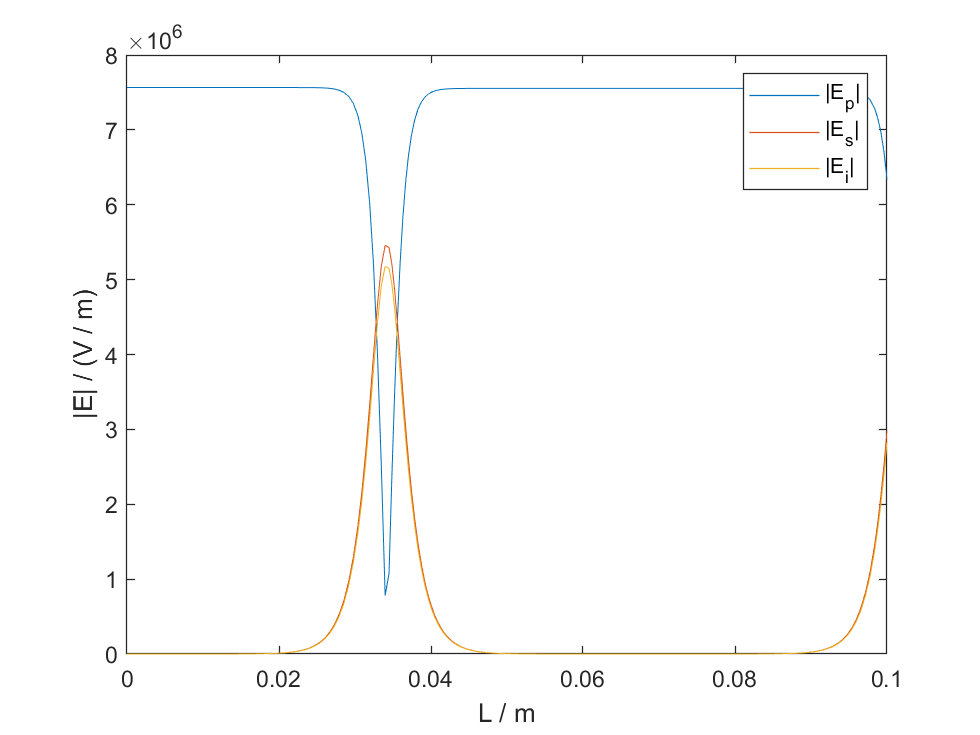
\includegraphics[width=.5\textwidth]{E-L.png}
        \caption{The magnitude of signal beam varying with the propagating distance}
        \label{E-L}
    \end{figure}

    At $L\approx 0.034$ m, the signal and the idler beam reached their maximum, so we should choose the length of the crystal to be $L=0.034\text{m}=34\text{mm}$.

    To avoid waste, we should make the cross section of the crystal as small as possible. Considering the divergence of the Gaussian beam, we should focus the beam waist to the center of the crystal. The Gaussian beam's cross section's radius at two ends of the crystal should be
    \begin{align}
        \nonumber w(L/2)=&w_0\sqrt{1+\left(\frac{\lambda_pL/2}{\pi w_0^2}\right)^2}=w_0\sqrt{1+\left[\frac{cL}{n(\omega_p)\omega_pw_0^2}\right]^2}=w_0\sqrt{1+\left[\frac{cL}{(n(\omega_s)\omega_s+n(\omega_i)\omega_i)w_0^2}\right]^2}\\
        =&0.05046\text{cm}\times\sqrt{1+\left[\frac{3\times 10^8\times 0.034}{3.915\times 10^{15}\text{rad}/\text{s}\times(0.05046\times 10^{-2})^2}\right]^2}=0.05047\text{cm}.
    \end{align}
    The cross section of the crystal should be
    \begin{align}
        A=\pi w^2(L/2)=0.00800\text{cm}^2=0.800\text{mm}^2.
    \end{align}


    \newpage
    \noindent\rule{\columnwidth}{1pt}\\
    \textbf{Conclusion}:
    \begin{table}[h]
        \centering
        \begin{tabular}{|c|c|c|}
            \hline
            Phase matching type & \multicolumn{2}{c|}{Type I} \\ \hline
            \multirow{3}{*}{Combination of the input and the output polarization directions} & signal & extraordinary \\ \cline{2-3} 
             & signal & ordinary \\ \cline{2-3} 
             & idler & ordinary \\ \hline
            \multirow{2}{*}{Orientation} & $\theta$ & $0.361$ rad \\ \cline{2-3} 
             & $\phi$ & $\frac{\pi}{3}$ rad \\ \hline
            Length & \multicolumn{2}{c|}{$34$ mm} \\ \hline
            Cross Section & \multicolumn{2}{c|}{$0.800$ mm$^2$} \\ \hline
        \end{tabular}
    \end{table}
\end{sol}

\noindent\rule{\columnwidth}{1pt}\\
\textbf{Appendix}\\
The code to find the proper length of the crystal:
\begin{lstlisting}
% main program
[T,E] = ode45('F',[0 0.1],[7565283.5547819445;1;0]);
plot(T,sqrt(conj(E(:,1)) .* E(:,1)))
hold on
plot(T,sqrt(conj(E(:,2)) .* E(:,2)))
plot(T,sqrt(conj(E(:,3)) .* E(:,3)))
xlabel('L / m')
ylabel('|E| / (V / m)')
legend('|E_p|','|E_s|','|E_i|')
\end{lstlisting}

\begin{lstlisting}
% write the following code in a file named 'F.m' and put the file in the same folder with the main program
function dE = F(t,E)
c = 3e8;
omega_p = 2.356194490192345e+15;
n_p = 1.6456018271928685;
omega_s = 1.240929098167968e+15;
n_s = 1.6470499268968157;
omega_i = 1.115265392024377e+15;
n_i = 1.6439905613250965;
d = 2.135e-12;
dE = [1i * 4 * pi * omega_p / n_p / c * d * E(2) * E(3); 1i * 4 * pi * omega_s / n_s / c * d * E(1) * conj(E(3)); 1i * 4 * pi * omega_i / n_i / c * d * E(1) * conj(E(2))];
\end{lstlisting}
\end{document}